\section{Architectures}
This first section will examine the various architectures that have been designed and synthesized for the floating point multiplier.

\subsection{Classic Architecture}
The starting point for the design was the 32-bit floating point pipelined multiplier, for which vhdl code was provided.
The outline scheme is shown in \autoref{fig:mult_struct}, it is divided into 4 main stages:
\begin{itemize}
\item Stage 1: The two input floating point numbers are unpacked.
\item Stage 2: Multiplication of significands, treated as integers, is carried out.
\item Stage 3: The rounding of significands is carried out.
\item Stage 4: The calculation of the exponent is carried out and finally the number is again transformed into a floating point through the packaging block.
\end{itemize}

\begin{figure}[h]
	\center
	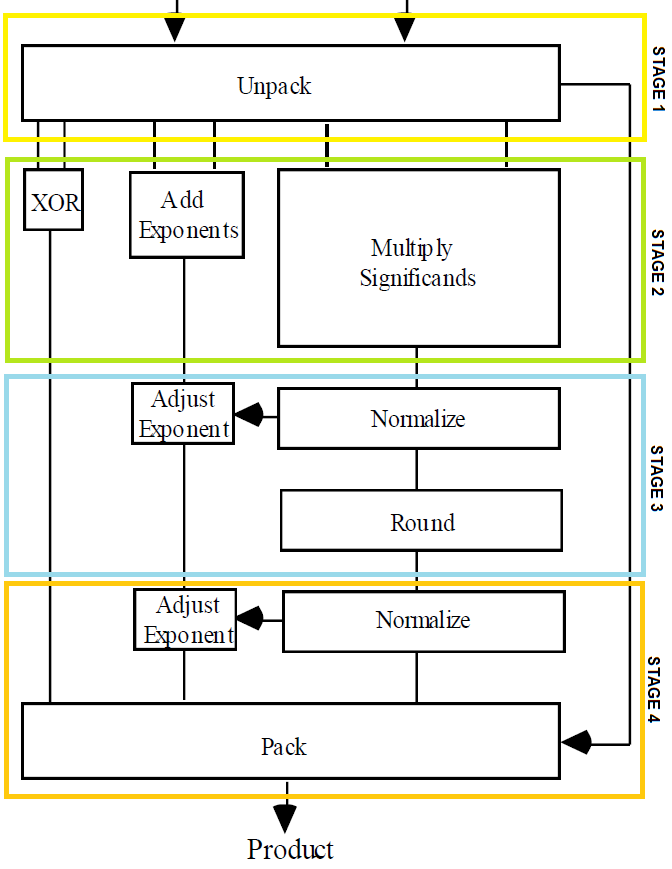
\includegraphics[width=0.6\textwidth]{mult_structure.png}
	\caption{Structure of the floating point multiplier}
	\label{fig:mult_struct}
\end{figure}

\noindent Studying the VHDL source, it can also be noticed that there are always registers between the stages which sample the signals on the rising edge of the clock. This is the reason why the functional stages correspond to the pipeline ones.
Moreover it is possible to observe that in the second stage the type of multiplier used to multiply the significands is not specified, in fact there is a process in which the operation is done with the symbol "*" which leaves the synthesizer the choice of hardware implementation.

\subsubsection{Testbench}
Before starting with the various hardware modifications, the correct functioning of the supplied circuit was simulated using Modelsim. For this purpose, a testbench was created in verilog with blocks for input generation, DUT and output saving.
The input file used is the one provided for both input $A$ and $B$ so the multiplier performs the square of the number in question. The numbers were represented on 8 hexadecimal bits, so conversion to binary was performed before feeding them to the DUT.
Finally, by comparing the results obtained with those provided as an example, it was possible to confirm the functioning of the circuit. Furthermore, by studying the timing generated by Modelsim, found in \autoref{fig:timing_standard}, it can be seen that the latency of the circuit is indeed as assumed, i.e. four clock strokes.

\begin{figure}[h]
	\center
	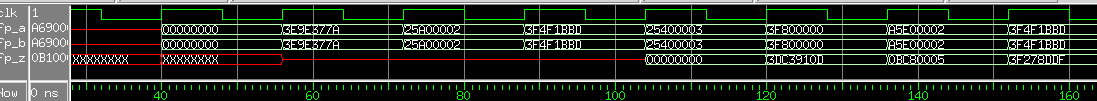
\includegraphics[width=1\textwidth]{timing_standard.png}
	\caption{Timing of the standard implementation}
	\label{fig:timing_standard}
\end{figure}

Afterwards, the VHDL code was modified so that registers were added to the input signals; this correction helps to decouple the timing of the inputs, with possible glitches, from the internal timing of the circuit, thus avoiding unexpected errors.
This modification was followed by a second testbench, which is functionally the same as the previous one, and again showed that the device under test worked correctly. As can be seen in \autoref{timing_reg} the only difference with the previous implementation is that the latency of the circuit increases by moving to five clock cycles.

\begin{figure}[h]
	\center
	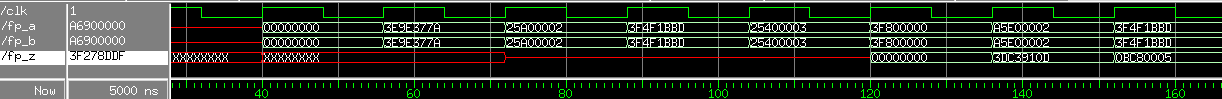
\includegraphics[width=1\textwidth]{timing_reg.png}
	\caption{Timing of the standard implementation with input registers}
	\label{fig:timing_reg}
\end{figure}

%%%%%%%%%%%%%%STAGE 2 MANIPULATION%%%%%%%%%%%%%%%


\subsection{Carry Save Adder (CSA)}
The Carry Save Adder is a 3 inputs and 2 otputs digital device, where the carry-in terminal has been replaced by a third general input. In fact, this device can be also used to sum in parallel three or plus different binary numbers, without lost of efficiency and excessive growing of area. \\
The basic single block is shown in the image below:

\begin{figure}[H]
	\center
	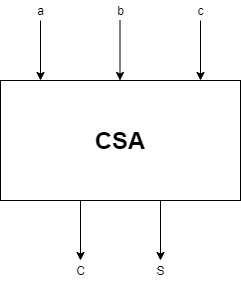
\includegraphics[width=0.3\textwidth]{CSA.png}
	\caption{Carry Save Adder basic block}
	\label{fig:CSA}
\end{figure}

In general, the \textit{carry save adder} block has no difference in terms of logic gates if compared to the \textit{full adder}, but they are used in a diffenent way. \\
The \textit{CSA} allows to compute some addition parts in parallel, and after, the partial results are combined in order to reach the complete summation of the numbers in input. The image below shows an example of the \textit{CSA tree}:
\begin{figure}[H]
	\center
	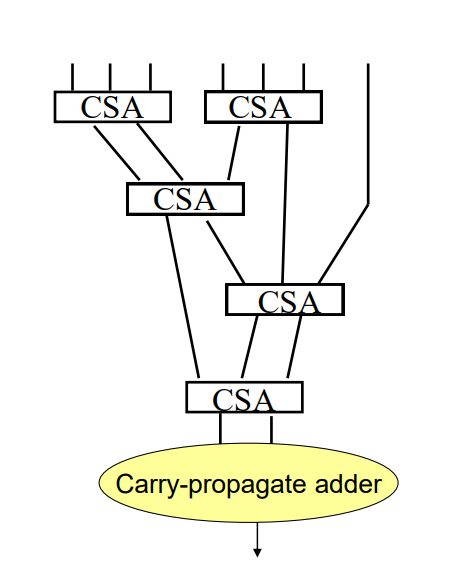
\includegraphics[width=0.35\textwidth]{CSA_tree.png}
	\caption{Carry Save Adder tree}
	\label{fig:CSA_tree}
\end{figure}
There are a lot of algorithms that exploit the power of this device, and there are several approaches used to speed up the execution of an addition or a multiplication, the mains are the Wallace and Dadda ones, this last will be analysed and simulated later, in this laboratory.
\subsection{Parallel Prefix Architecture (PPARCH)}
In this section a few optimizations was done. In fact, respect to the classic architecture there are several differences that change the circuit behavior. The CSA architecture is implemented by using the \textit{Carry Save Adders} and in the PPARCH architecture there is a \textit{pipelined} version of the stage 2. These variations can be carried out by simply using different commands during the compilation process. The stage 2 was forced to be syntetized as CSA and to do that the following commands were used in the synthesis process:


The \textit{PPARCH} analysed in this lab has been previously improved by using two particular techniques: the \textit{carry look ahead} and the \textit{parallel prefix}. The first one uses a combination of \textit{generate} and \textit{propagate} to compute the carries faster than a \textit{ripple carry adder} architecture. Generate and Propagate are computed by combinating the binary input signals:
\begin{itemize} 
\item Generate $G_i = A_i \cdot B_i$
\item Propagate $P_i = A_i \oplus B_i$
\end{itemize}
By using these signals is possible to compute the carries and the partial sums:
\begin{center}
$C_{i+1} = G_i + P_i \cdot C_i$ \\
$S_i = P_i \oplus C_i $
\end{center}
In particular, it's possible to unroll the carries equation, in order to speed up the computation:

\noindent
$C_0 = C_0$ \\
$C_1 = G_0 + P_0 \cdot C_0$\\
$C_2 = G_1 + P_1 \cdot C_1 = G_1 + G_0 \cdot P_1  + P_1 \cdot P_0 \cdot C_0$\\
and in general: \\
$C_i = G_{i-1} + P_{i-1} \cdot C_{i-1}$\\
\noindent
All these computations require a lot of hardware to be computed and there is an issue called a \textit{Parallel Prefix} problem: the generate-propagate network can be very long and this can develop problem in terms of the critical path. In fact, a several algorithm has been invented in order to improve the performance of this newtork, for example: Kogge-Stone , Ladner-Fishner, Brent-Kung. Synopsys can arbitrarily use one these optimizations in order to minimize the hardware required to develop the generate-propagate carry generation network.
\subsection{Stage 2 CSA PPARCH}
In this section a few optimizations were done. In fact, compared to the classic architecture there are several differences that change the circuit behavior. The CSA architecture is implemented by using the \textit{Carry Save Adders} and in the PPARCH architecture there is a \textit{Parallel Prefix} version of the stage 2. These variations can be simply carried out by using different commands during the compilation process. The stage 2 was forced to be syntetized as CSA and in order to do that the following commands were used in the synthesis process:

\begin{itemize}
\item ungroup -all flatten
\item set\_implementation DW02\_mult/csa [find cell *mult]
\end{itemize}
For the PPARCH the same commands were used, but with one difference in the mult options:
\begin{itemize}
\item ungroup -all flatten
\item set\_implementation DW02\_mult/pparch [find cell *mult]
\end{itemize}
The goals of the synthesis process was the area and the minimum period estimation and the results obtained from the commands \textit{report\_area} e \textit{report\_timing} are showed in \autoref{tab:syn_results}: the \textit{CSA} architecture is roughly three times slower and the area is much greater than the \textit{PPARCH} one and the \textit{PPARCH} is a better architecture respect to the \textit{CSA} one.
To check the correct behavior, a testbench was performed on both architectures, and the otuput is shown in the following table:

\begin{table}[H]
\begin{center}
\begin{tabular}{cc}				
CSA		 	  & PPARCH 					\\ \hline
00000000   	  & 00000000               	\\ 
3DC3910D      & 3DC3910D                \\ 
0BC80005      & 0BC80005                \\ 
3F278DDF      & 3F278DDF                \\ 
0B100005      & 0B100005                  \\ 
3F800000      & 3F800000              \\ 
0C440004      & 0C440004 
\end{tabular}
\end{center}
\end{table}
As the table illustrates, the behavior of both architecture is the same; in addiction, once the input stream reaches the end of file, the output remains the same as long as the simulation runs, in fact the output remains equal to the string \textit{3DC3910D}. In conclusion both architectures work, but in a different way due to the internal structure.

%%%%%%%%%FINE-GRAIN PIPELINING%%%%%%%%%%%%%

\subsection{Fine grain pipelining}
The next aim is to modify the VHDL file by inserting a \textit{pipeline stage} in stage 2 output, as shown in the following image:
\begin{figure}[htb]
	\center
	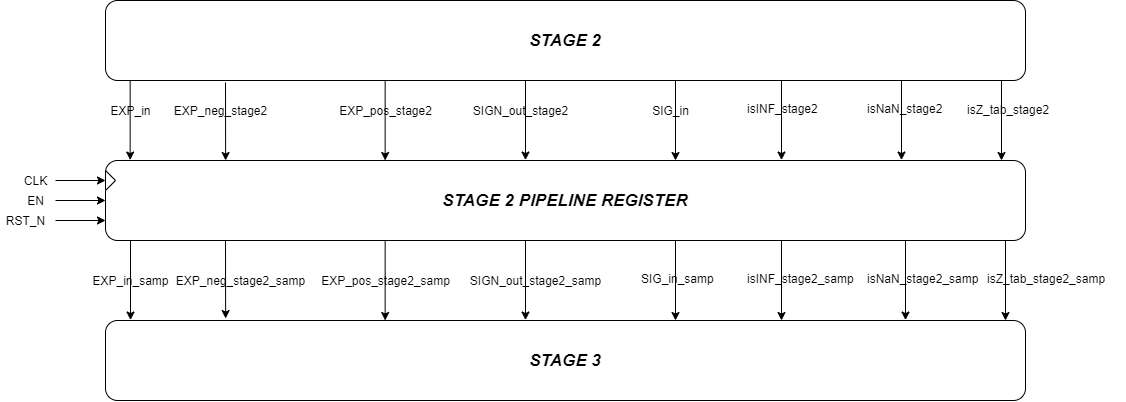
\includegraphics[width=0.9\textwidth]{Fine grain pipelining.png}
	\caption{Fine grain pipelining block diagram}
	\label{fig:fine_pipe}
\end{figure}
The output register has been implemented in the VHDL file by using several registers in order to ensure the correct behavior and timing.  After the VHDL manipulation, two different synthesis processes were made by using different commands per time: in the first run, the compile command was launched after \textit{optimize\_registers} command and in the second run  \textit{compile\_ultra} was used rather than \textit{optimize\_registers} and \textit{compile}. The Synthetizer elaborates the structures in a different way, by using some algorithms instead of other ones, according to the choosen command. The results in terms of timing and area are showed in \autoref{tab:syn_results}: the \textit{compile\_ultra} give a lower area but the circuit is clearly slower respect to the one obtained by using \textit{optimize\_registers}.

\subsubsection{Testbench}
To verify the correct behaviour, a Modelsim simulation was launched prior to the synthesis, which again showed proper functioning. As can be seen in \autoref{fig:timing_fine_grain} the latency of the circuit is correctly increased by changing to six clock cycles.

\begin{figure}[h]
	\center
	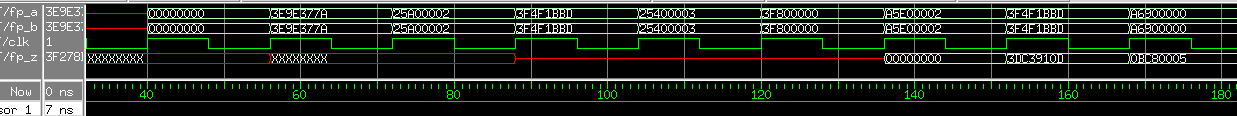
\includegraphics[width=1\textwidth]{timing_fine_grain.png}
	\caption{Timing of the fine grain pipelining implementation}
	\label{fig:timing_fine_grain}
\end{figure}


\subsection{Modified Booth Encoding (MBE)}
The Modified Booth Encoding Multiplier is an extension of the Radix-2 approach, where a Radix-4 approach is used in order to produce half partial products. In generale considerando \textbf{a} e \textbf{b} come due numeri unsigned nella forma seguente:
$$
\textbf{a} = \sum_{i=0}^{n-1}a_i2^i\ \ \ \ \ \ \  \textbf{b} = \sum_{i=0}^{n-1}b_i2^i
$$
The product \textbf{c} is obtained:
$$
\textbf{c} = \sum_{i=0}^{n-1}\sum_{i=0}^{n-1}a_ib_i2^{i+j}
$$
Radix-2 approach produces \textbf{n} partial products in the form:
$$
p_j =
\begin{cases}
0 \ \textrm{  if   } \overline{b}_j\\
a \ \textrm{  if   } {b}_j
\end{cases}
$$
On the other hand MBE produces only \textbf{n/2} partial products because more bits are analyzed simultaneously. The multiplier is divided in 3-bit slices (with $b_{-1} = 0$), where two consecutive slices feature a 1-bit overlap. Then, each triplet of bits is exploited to encode the multiplicand according to the \autoref{tab:MBE}.
\begin{table}[htb]
	\centering
	\begin{tabular}{cc}
		$b_{2j+1}b_{2j}b_{2j-1}$ & $p_j$ \\
		\hline
		000 & 0 \\
		001 & a \\
		010 & a \\
		011 & 2a \\
		100 & -2a \\
		101 & -a \\
		110 & -a \\
		111 & 0 \\
	\end{tabular}
	\label{tab:MBE}
	\caption{Modified Booth Encoding}
\end{table}
The expression to evaluate $p_j$ is $p_j = (b_{2j+1} \oplus q_j) + b_{2j+1}$ where
$$ q_j=
\begin{cases}
0 \ \textbf{  if   } (\overline{b_{2j} \oplus b_{2j-1}})(\overline{b_{2j+1} \oplus b_{2j}})\\
a \ \textbf{  if   } b_{2j} \oplus b_{2j-1}\\
2a \ \textbf{  if   } (\overline{b_{2j} \oplus b_{2j-1}})(b_{2j+1} \oplus b_{2j})
\end{cases}
$$
A total of 16 combinatorial blocks were used to evaluate all partial products that have to be summed. An overview of the structure with a dot view can be seen in \autoref{fig:Dadda_1}.
\begin{figure}[htb]
	\center
	
\includegraphics[width=1\textwidth]{Dadda_Tree_1.png}
	\caption{Partial products representation}
	\label{fig:Dadda_1}
\end{figure}
A Dadda Tree was used to cover the bits in order to use an optimal number of stages and thus high speed in performing the operations. The approach is to reduce the height at each stage until a predetermined number of bits is reached using half-adders and full-adders. The heights follow the sequence:
$$
d_1 = 2 \ \ \ \ \ \ \ \ d_{j+1} = \lfloor(1.5d_j)\rfloor
$$
The initial height of the structure is 16, so the sequence will be:
$$
d_1 = 2,\ d_2 = 3,\ d_3 = 4,\
d_4 = 6,\ d_5 = 9,\ d_6 = 13,\ d_7 = 16
$$
Since the next step has a height of 13, all columns that have a higher number of bits must be reduced. Starting from the right, on the first column that has 14 bits a half-adder has been inserted that starting from two bits generates a new bit on the same column and a carry bit on the next column. The adjacent column that still has 14 bits, considering the carry from the previous half-adder, requires a full-adder which, from three bits, generates a sum bit on the same column and a carry bit on the next column. This reasoning has been repeated on the whole structure and the final result can be observed in \autoref{fig:Dadda_1} where 6 half-adders (in orange) and 33 full-adders (in green) have been used.
The same mechanism is applied to each stage to reduce the number of bits while respecting the sequence. In \autoref{fig:Dadda_2} it is possible to observe the coverage of each stage up to a height of two bits, where thanks to a adder the final result can be computed.
\begin{figure}[htb]
	\center
	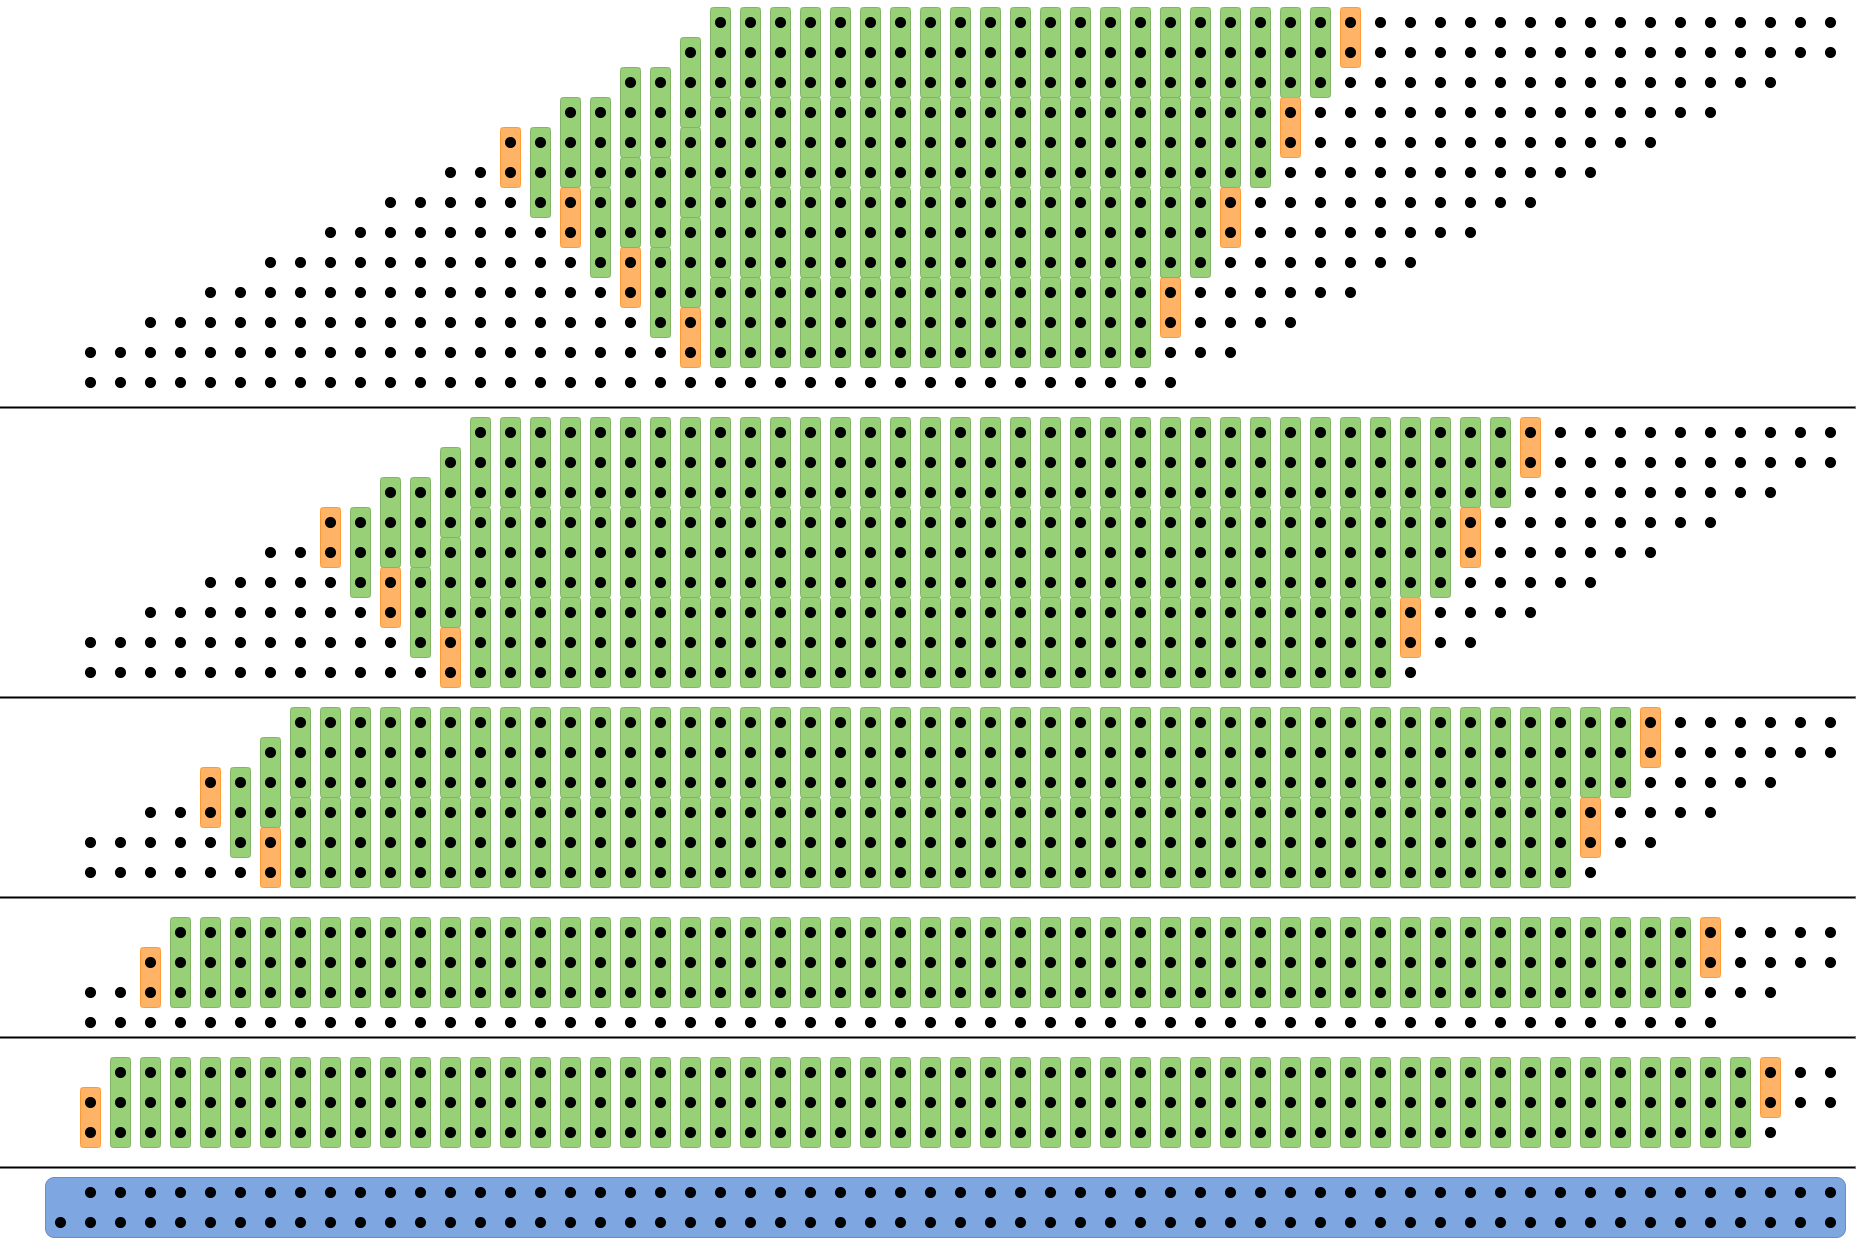
\includegraphics[width=1\textwidth]{Dadda_Tree_2.png}
	\caption{Dadda Tree }
	\label{fig:Dadda_2}
\end{figure}
The number of half-adders and full-adders for each stage are summarized in \autoref{tab:adders_count}. The last stage can be implemented in different ways; to get an idea of the final result it has been considered as a ripple-carry adder.
\begin{table}[htb!]
	\centering
	\begin{tabular}{ccc}
		stage & HA & FA \\
		\hline
		1 & 6 & 33\\
		2 & 8 & 84\\
		3 & 6 & 105\\
		4 & 4 & 90\\
		5 & 2 & 51\\
		6 & 2 & 55\\
		7 & 2 & 58\\
		Tot & 30 & 476\\
	\end{tabular}
	\label{tab:adders_count}
	\caption{Number of adders used}
\end{table}
Once the structure was defined a program written in C++ \footnote{\href{https://github.com/HSOgawa/fast-multipliers}{\textcolor{black}{Source: } here}} \thispagestyle{empty}, was used to generate the vhdl code related to the MBE multiplier.

\pagebreak
\subsubsection{Testbench}
The correct functioning of the circuit was verified using the previously written testbench. Comparing the results obtained with those expected has confirmed the correctness of the implementation and when looking at the timing no differences were noticed compared to \autoref{fig:timing_reg}.
\pagebreak